\author{Марухленко Д.С. @japersik}
\date{\today}

\documentclass[a4paper,12pt]{article}
\usepackage[english,russian]{babel}
\usepackage[utf8]{inputenc}
\usepackage{amsmath,amsfonts,amssymb,amsthm,mathtools}
\usepackage{hyperref}
\usepackage{wrapfig}

\usepackage[left=2.5cm, right=1.5cm, top=2.5cm, bottom=2.5cm]{geometry}
\usepackage{array}
\usepackage{tabularx}
\usepackage{indentfirst}
\usepackage{stmaryrd}
\usepackage{graphicx}
\setlength\parindent{5ex}

\usepackage{fancyhdr} %%колонтикулы
\usepackage{lastpage}
\pagestyle{fancy}
\fancyhf{}
\rfoot{\thepage}
\cfoot{}
\lfoot{}
\renewcommand{\footrulewidth}{0.4pt}

\usepackage{lipsum}
\usepackage{wasysym}
\usepackage{booktabs}
\usepackage{blindtext}
\usepackage{siunitx}% provides filler text


\usepackage{svg}

\newcommand{\authorName}{Марухленко Д.С.\\Попов Н.А.\\Андриянов В.А\\Полит А.Д}
\newcommand{\workType}{Лабораторная работа №3}
\newcommand{\workName}{Исследование бесконтактных датчиков приближения}
\newcommand{\subjectName}{Преобразователи информации}
\newcommand{\workOption}{Вариант №6}
\newcommand{\groupNumber}{R34352}
\newcommand{\teacherName}{Быстров С.В}

\begin{document}
    \thispagestyle{empty}
%титульный лист%
\begin{center}
    Национальный исследовательский университет ИТМО\\
    Факультет систем управления и робототехники
    \vskip 7cm

    \Huge \workType                         \\
    \huge <<\workName>>                     \\
    \Large по дисциплине <<\subjectName>>   \\
\end{center}
\vfill

\begin{flushright}
    Подготовили: \authorName         \\
    Группа: \groupNumber            \\
    Преподаватель: \teacherName     \\
\end{flushright}
\vskip 2cm

\begin{center}
    Санкт-Петербург 2022г.
\end{center}
\newpage
    \section{Цель работы}
Ознакомление с устройством бесконтактных датчиков приближения, изучение принципов работы и схем включения.
    \section{Марериалы работы}

\subsection{Основные технические характеристики исследуемого датчика}
Исследуемый датчик -- инкрементальный энкодер.
Относится к типу энкодеров, которые предназначены для указания направления движения и/или углового перемещения внешнего механизма.
Инкрементальный энкодер формирует импульсы, количество которых соответствует повороту вала на определенный угол.
Этот тип энкодеров, в отличие от абсолютных, не формирует код положения вала, когда вал находится в покое..

Паспортные характеристики исследуемого энкодера E50S8:
\begin{itemize}
    \item Диаметр корпуса: 50 мм
    \item Диаметр вала: 8 мм
    \item Количество импульсов на оборот вала: 1000
    \item Выходной сигнал: дифференциальный, парафазный
    \item Напряжение питания: 5В постоянного тока
\end{itemize}

\subsection{Экспериментальная установка и змерительные средства}
Помимо прочего, блок содержит приводной двигатель постоянного тока и энкодер, соединенные зубчатой передачей.
\begin{figure}[!h]
    \centering
    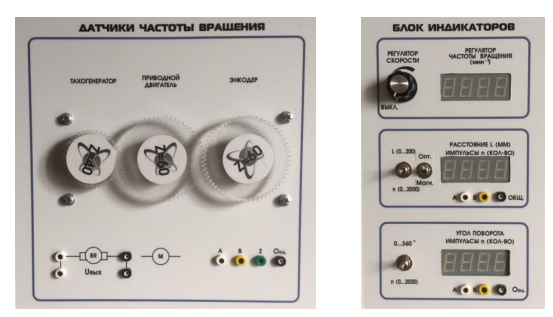
\includegraphics[width=0.8\textwidth]{img/Screenshot_20221002_213647}
    \caption{Панель экспериментальной установки}
    \label{fig:Screenshot_20221002_213647}
\end{figure}

Угол поворота энкодера и количество импульсов отображаются на одном (нижнем) индикаторном блоке.
Переключение режимов отображения осуществляется тумблером.

\subsection{Результаты измерений и их обработка}
Зафиксируем статическую характеристику энкодера на холостом ходу.
\begin{table}[!h]
    \centering
    \caption{Статическая характеристика энкодера}
    \label{tab:tabl}
    \begin{tabular}{|c|c|}
        \hline
        Угол поворота $\alpha,^\circ$& Число импульсов $N$ \\\hline
        0&	0\\
        30&	84\\
        60&	169\\
        90&	252\\
        120&	335\\
        150&	417\\
        180&	502\\
        210&	584\\
        240&	669\\
        270&	751\\
        300&	835\\
        330&	919\\
        360&	1000\\
        \hline
    \end{tabular}
\end{table}

Построим график:

\begin{figure}[!h]
    \centering
    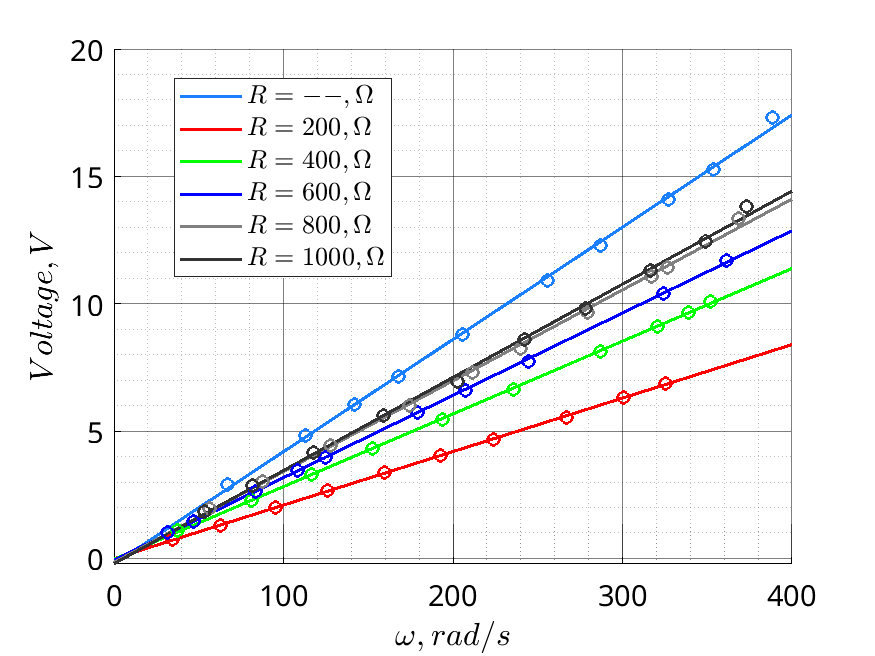
\includegraphics[width=0.8\textwidth]{img/task1_r_0}
    \caption{Статическая характеристика энкодера }
    \label{fig:task1_r_0}
\end{figure}

\subsection{Расчет погрешностей}
Найдем максимальное значение абсолютной и относительной погрешностей:
\begin{table}[!h]
    \centering
    \label{tab:otkl}
    \begin{tabular}{|c|c|}
        \hline
        Наибольшая $\Delta N$ & $\epsilon,\%$\\        \hline
        2.33& 1.4\\ \hline
    \end{tabular}
    \caption{Значения погрешностей}

\end{table}

\newpage
\section{Вывод}
В ходе работы мы на практике поработали с инкрементальным энкодером и построена его статическая характеристика.
Было установлено, что статическая характеристика энкодера линейная.
\end{document}